\begin{center}
\makeatletter
\@ifundefined{color@atlasink}{\definecolor{atlasink}{HTML}{33312E}}{}
\@ifundefined{color@atlasgray}{\definecolor{atlasgray}{HTML}{9A958C}}{}
\@ifundefined{color@atlasblue}{\definecolor{atlasblue}{HTML}{2E6F9E}}{}
\@ifundefined{color@atlasgreen}{\definecolor{atlasgreen}{HTML}{4C8C3F}}{}
\@ifundefined{color@atlasred}{\definecolor{atlasred}{HTML}{C0473B}}{}
\@ifundefined{color@atlasgold}{\definecolor{atlasgold}{HTML}{D69A2A}}{}
\@ifundefined{atlascaption}{%
  \newcommand{\atlascaption}[3]{\shortstack{\footnotesize Figure~#1. \textbf{#2:}\\#3}}%
}{}
\@ifundefined{glowstroke}{%
  \newcommand{\glowstroke}[3]{%
    \draw[#1, line width=1.5pt, line cap=round]
      plot[domain=#2,samples=100,smooth] (\x,{#3});%
  }%
}{}
\makeatother
\tikzset{
  atlas axes/.style={atlasink, line width=0.7pt, line cap=round, ->},
  atlas curve/.style={line width=1.5pt, line cap=round, line join=round},
  dropline/.style={atlasgray, line width=0.6pt, dash pattern=on 2pt off 2pt},
  atlas dot/.style={fill=atlasink, draw=white, line width=0.4pt, circle, inner sep=0pt, minimum size=4.2pt},
}

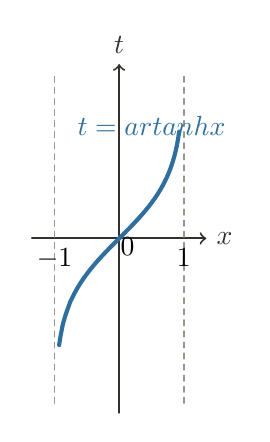
\begin{tikzpicture}[scale=0.82, line cap=round, line join=round]
  \draw[atlas axes] (-1.35,0)--(1.35,0) node[right] {$x$};
  \draw[atlas axes] (0,-2.7)--(0,2.7) node[above] {$t$};
  \draw[dropline] (-1,-2.55)--(-1,2.55);
  \draw[dropline] (1,-2.55)--(1,2.55);
  \glowstroke{atlasblue}{-0.93:0.93}{0.5*ln((1+\x)/(1-\x))}
  \fill[atlas dot] (0,0) node[below right] {$0$};
  \node[below] at (-1,0) {$-1$};
  \node[below] at (1,0) {$1$};
  \node[atlasblue] at (0.5,1.75) {$t=\operatorname{artanh}x$};
\end{tikzpicture}

\atlascaption{HI3}{Inverse hyperbolic tangent}{Domain $(-1,1)$ and range $\mathbb{R}$; the vertical lines $x=\pm 1$ are asymptotes.}
\end{center}


\begin{definitionbox}{Definition}
\begin{definition}[Inverse hyperbolic tangent]
\label{def:inverse-hyperbolic-tangent}
The \emph{inverse hyperbolic tangent} function is the inverse of $\tanh$ on
its full domain. It is denoted by $\operatorname{artanh}$ and has domain
$(-1,1)$ and range $\mathbb{R}$.
\[
  \operatorname{artanh} x=t
  \quad\Longleftrightarrow\quad
  \tanh t=x.
\]
\end{definition}
\end{definitionbox}
\begin{remark*}[Standard quantified statement]
For every admissible input satisfying the hypotheses of the statement, the
displayed definition or assertion holds in the stated domain.
\end{remark*}

\begin{remark*}[Interpretation]
The statement records the named trigonometric object or identity together with
its intended domain of use.
\end{remark*}

\begin{remark*}[Domain and range]
The regular function $\tanh:\mathbb{R}\to(-1,1)$ is strictly increasing.
Its horizontal asymptotes show that the endpoint values $-1$ and $1$ are not
attained, so they are not in the inverse domain.
\end{remark*}
\begin{dependencies}
\begin{itemize}
  \item \hyperref[def:hyperbolic-tangent]{Hyperbolic tangent}
\end{itemize}
\end{dependencies}

\begin{theorembox}{Theorem}
\begin{theorem}[Principal inverse hyperbolic tangent identities]
\label{thm:inverse-hyperbolic-tangent-identities}
For every $x\in(-1,1)$,
\[
  \tanh(\operatorname{artanh} x)=x.
\]
For every $t\in\mathbb{R}$,
\[
  \operatorname{artanh}(\tanh t)=t.
\]
\end{theorem}
\end{theorembox}
\begin{remark*}[Standard quantified statement]
For every admissible input satisfying the hypotheses of the statement, the
displayed definition or assertion holds in the stated domain.
\end{remark*}

\begin{remark*}[Interpretation]
The statement records the named trigonometric object or identity together with
its intended domain of use.
\end{remark*}

\begin{remark*}[Proof]
Both identities are the cancellation laws for the inverse of
$\tanh:\mathbb{R}\to(-1,1)$.
\end{remark*}
\begin{dependencies}
\begin{itemize}
  \item \hyperref[def:inverse-hyperbolic-tangent]{Inverse hyperbolic tangent}
\end{itemize}
\end{dependencies}
